\chapter{Controlador de corriente} \chapterlabel{Informe/4-ControladorCorriente} \label{cap:ControladorCorriente}

En este capítulo se diseña y modela el circuito encargado de controlar la corriente que circula por el electroimán. Como se vio en el capítulo anterior, el sistema trabaja con corrientes elevadas por lo que se implementan estrategias de conmutación para reducir las pérdidas de energía. Para ello se utiliza una topología de puente H con cuatro MOSFET y un \textsl{driver} que los controla. Además, se detallan los criterios tenidos en cuenta al momento de  elegir  y dimensionar todos los componentes que intervienen para lograr el correcto funcionamiento del controlador de corriente. Por último, se obtiene su función transferencia  para ser utilizada en el diseño del compensador.

\section{Descripción general}\label{sec_descripcion-general}

Para mantener en suspensión a la pieza móvil es necesario regular la fuerza electromagnética generada por el electroimán. Esto se logra modificando la intensidad de la corriente que circula por su bobinado como lo indica la expresión \ref{eq_fuerza_magnetica}. Por lo tanto, es necesario diseñar una fuente de alimentación que sea capaz de proveer la corriente requerida. 

Como se analizó en el capítulo \ref{cap:CaracterizacionElectroiman}, el electroimán puede ser modelado como una inductancia que varía con la distancia de entrehierro y una resistencia serie. Es decir, como un circuito RL serie cuya admitancia se muestra en la expresión \ref{eq_corriente}.

\begin{equation} \label{eq_corriente}
\frac{I_L}{V_L}(s)=\frac{1}{sL(Y_g)\ +\ R_L}
\end{equation}

Al aplicar la transformada inversa de Laplace a la expresión  \ref{eq_corriente}, se obtiene la respuesta temporal de la corriente ante un escalón de tensión con amplitud $v_L$ en la entrada, considerando corriente inicial $I_o$ y constante de tiempo $\tau=\frac{L(Y_g)}{R_L}$.

\begin{equation} \label{eq_corriente_temporal_cond_iniciales}
	i_L(t)=\frac{v_L}{R_L} + (I_o-\frac{v_L}{R_L})*e^{-\frac{t}{\tau}}
\end{equation}

En la expresión \ref{eq_corriente_temporal_cond_iniciales} se puede observar que la respuesta al escalón está compuesta por dos partes: un término con una exponencial negativa correspondiente al transitorio, y un término constante correspondiente al valor en régimen permanente $\frac{v_L}{R_L}$. El primero es el responsable de que la corriente en el inductor crezca de manera amortiguada, hasta alcanzar el valor de régimen permanente luego de cierto tiempo. Este comportamiento se puede observar en la simulación realizada en la figura \ref{fig:img_respuesta_escalon}. En la parte superior se observa la tensión de entrada y, en la inferior, la corriente del electroimán. Este análisis resulta de utilidad para conocer el comportamiento del electroimán y diseñar un controlador de corriente adecuado.


\begin{figure}[H]
	\centering
	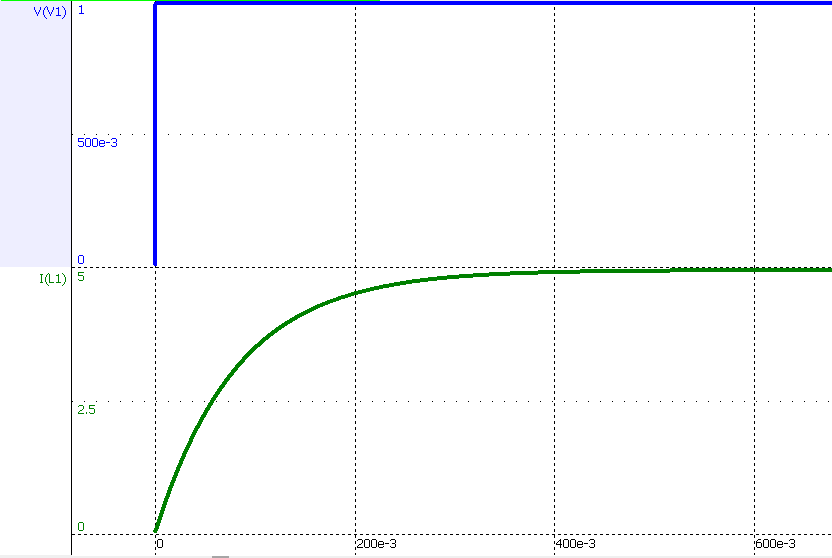
\includegraphics[scale=0.5]{corriente_escalon.png}
	\caption{Respuesta ante una entrada en escalón.}
	\label{fig:img_respuesta_escalon}
\end{figure}


\section{Diseño del controlador}


Se desea diseñar un sistema de control que modifique la alimentación del electroimán con el objetivo de que circule una corriente con un valor medio deseado por su bobinado.  Para ello, se propone implementar un sistema realimentado que compare la corriente que circula por el electroimán con una de referencia, que es la que se desea que circule. En la figura \ref{fig:img_diagrama_bloques_basico} se muestra un diagrama en bloques simplificado del sistema.

\begin{figure}[H]
	\centering
	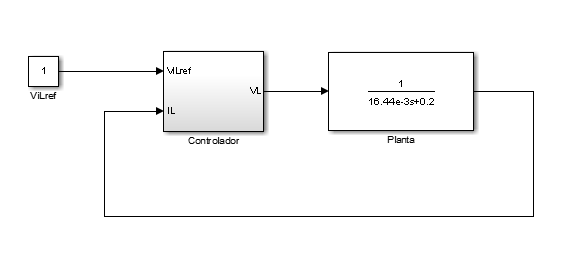
\includegraphics[scale=0.4]{Diagrama-en-bloques-basico.png}
	\caption{Diagrama en bloques básico del controlador de corriente.}
	\label{fig:img_diagrama_bloques_basico}
\end{figure}

\colorbox{red}{Está bien decir que del diagrama surge esto? No debería ser al revés?}

Del diagrama \ref{fig:img_diagrama_bloques_basico} surgen las siguientes necesidades:
\begin{itemize}
	\item Diseñar la topología de la fuente de alimentación.
	\item Diseñar un controlador que modifique la corriente que circula por el electroimán según sus entradas.	
	\item Medir la corriente que circula en el electroimán para poder utilizarla como entrada al controlador.
\end{itemize}

A continuación se analizan distintas alternativas para satisfacer cada una de las necesidades planteadas.

\subsection{Diseño de la topología de la fuente de alimentación}
En esta sección se analizan distintas topologías para la fuente de alimentación del electroimán. Inicialmente se analiza el funcionamiento de un controlador de corriente mediante el uso de un transistor trabajando en modo lineal y luego utilizando una fuente de alimentación trabajando en conmutación.

\subsubsection{Control de corriente mediante transistor en modo lineal}
Como se analizó en la sección \ref{sec_descripcion-general}, el valor en régimen permanente de la corriente depende proporcionalmente de la tensión aplicada al electroimán. Por lo tanto, para mantener una corriente constante controlada se podría utilizar un transistor en modo lineal como se muestra en el circuito de la figura \ref{fig:img_controlador-lineal}.

\begin{figure}[H]
	\centering
	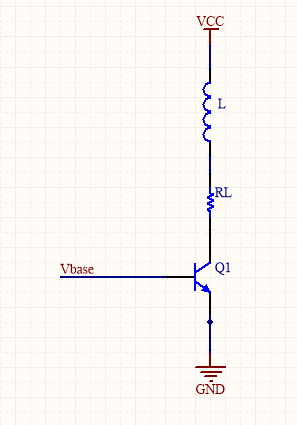
\includegraphics[scale=0.7]{controlador_lineal.png}
	\caption{Control de corriente mediante transistor en modo lineal.}
	\label{fig:img_controlador-lineal}
\end{figure}

En este modo de funcionamiento la tensión colector-emisor ($V_{CE}$) se controla de manera que su diferencia con la tensión de alimentación, al ser aplicada en los bornes del electroimán, genere la corriente deseada. Es decir, en régimen permanente se obtiene:
 
 \begin{equation}
 	I_L=\frac{V_{CC}-V_{CE}}{R_L}
 \end{equation}


Al considerar que la caída de tensión sobre el inductor es prácticamente nula (solo lo correspondiente a la resistencia interna), la mayor parte de la potencia disipada se produce en el transistor. Esta puede calcularse como: 

\begin{equation}
	P_{transistor} = I_L*V_{CE}
\end{equation}

Teniendo en cuenta que la tensión colector-emisor es la resta de la tensión de alimentación y la caída en la resistencia del electroimán:

\begin{equation}
	V_{CE}=V_{CC}-I_L*R_L
\end{equation}

Finalmente:

\begin{equation}
	P_{transistor}=V_{CC}*I_L-I_L^2*R_L
	\label{eq_p-transistor_lineal}
\end{equation}

La función \ref{eq_p-transistor_lineal} presenta un máximo cuando $I_L=\frac{V_{CC}}{2*R_L}$.


\begin{equation}\label{eq_pot_transistor_lineal_final}
	P_{transistor_{max}}=\frac{V_{CC}^2}{4*R_L}
\end{equation}


Teniendo en cuenta que la corriente máxima requerida es de aproximadamente $30\:A$ se obtiene que la mínima tensión de $V_{CC}$ es:

\begin{equation}\label{eq_vcc-min}
	V_{CC}=I_L*R_L+V_{CE}=30 A * 0,2  = 5 V, \:V_{CE}=0
\end{equation}

\colorbox{red}{es necesario poner esto de arriba? lo de la tensión mínima..}

En la ecuación \ref{eq_pot_transistor_lineal_final} se puede ver que para valores de tensión normalmente utilizados $(5\:V,10\:V,15\:V)$ la potencia disipada por el transistor varía entre $30\:W$ hasta $280\:W$. Esto eleva demasiado la temperatura del transistor y pone en riesgo la vida útil de los componentes, haciendo que sea necesario el agregado de un gran disipador de calor. Por este motivo, se procede a analizar otra alternativa para el diseño de la fuente de alimentación.

\subsubsection{Control de corriente mediante conmutación}

Como se analizó previamente, al trabajar con corrientes elevadas, no es eficiente utilizar un transistor que trabaje en su zona lineal puesto que el consumo de energía es elevado. Se propone entonces utilizar una fuente conmutada.

%\noindent Para lograr una corriente continua en el electroimán mediante una fuente conmutada se debe alternar la polaridad de la tensión aplicada en sus bornes. De esta forma, se aprovecha el transitorio mostrado en la figura \ref{fig:img_respuesta_escalon} para hacer crecer la corriente hasta llegar a un cierto valor (denominado límite superior), y luego se conmuta la polaridad de la alimentación para que decrezca. Nuevamente, al llegar a un cierto valor (denominado límite inferior), se vuelve a conmutar. Este proceso se repite, y se logra que la corriente oscile en torno al valor medio entre los dos límites, que es el valor de corriente continua deseado. 

Al aplicar tensión en los bornes del electroimán, la magnitud de la corriente aumentará en forma exponencial. Si se desea que la corriente que circule por su bobinado sea aproximadamente continua, es posible alternar la polaridad de la tensión aplicada ($\pm V_L$) de forma que la corriente oscile en torno al valor medio deseado ($<I_L>$) como se observa en la figura \ref{fig:img_corriente_exponencial}.

\begin{figure}[H]
	\centering
	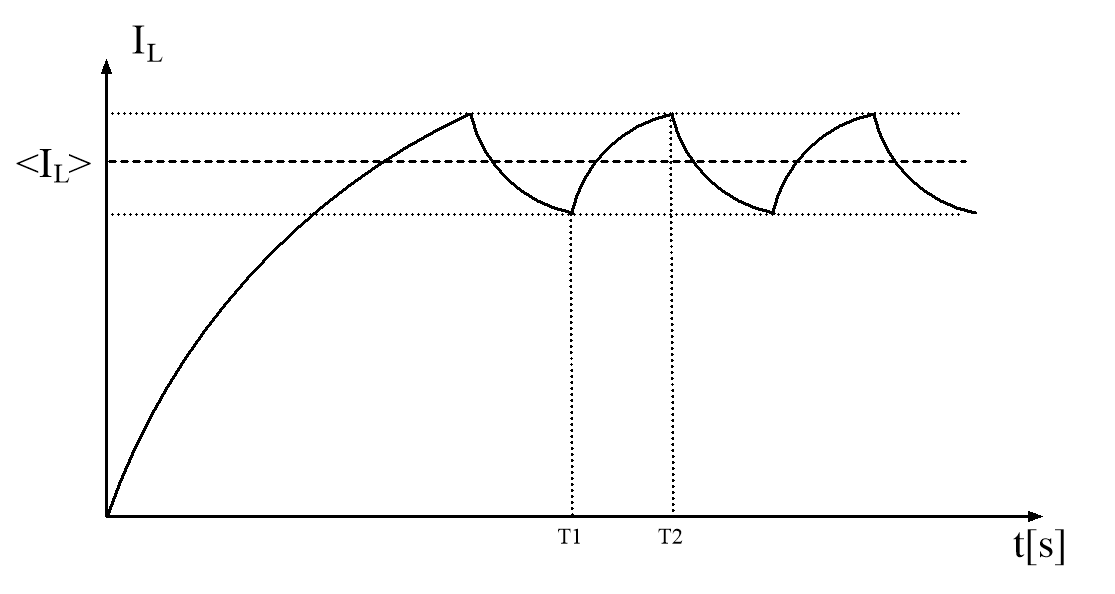
\includegraphics[scale=0.5]{Forma-de-onda-corriente-exponencial.png}
	\caption{Forma de onda de corriente y tensión en el electroimán.}
	\label{fig:img_corriente_exponencial}
\end{figure}

%En la figura \ref{fig:img_corriente_exponencial} se puede ver que la corriente crece y decrece en forma exponencial dentro de cada ciclo de conmutación. Sin embargo, si se elige un intervalo de tiempo de la conmutación pequeño comparado con la constante de tiempo de la planta, el incremento de corriente será pequeño y puede ser aproximado como una rampa. Por lo tanto, se obtiene una corriente continua con un ripple superpuesto de forma triangular, como la que se muestra en la figura \label{fig:img_corriente_lineal}.

%\begin{figure}[H]
%	\centering
%	\includegraphics[scale=0.5]{forma-de-onda-corriente-lineal.png}
%	\caption{Forma de onda de corriente al disminuir el período de conmutación.}
%	\label{fig:img_corriente_lineal}
%\end{figure}

Por lo tanto, es necesario diseñar un circuito que permita alternar la polaridad de la tensión aplicada al electroimán y controlar, de esta forma, el valor medio de su corriente. Entre las distintas topologías de fuentes conmutadas que se utilizan comúnmente, una que tiene la capacidad de alimentar su carga en ambos sentidos es la topología de puente completo con cuatro llaves que se muestra en la figura \ref{fig:img_topologia_simplificada}.

\colorbox{red}{vale la pena mencionar que alimenta la carga en ambos sentidos?}

\begin{figure}[H]
	\centering
	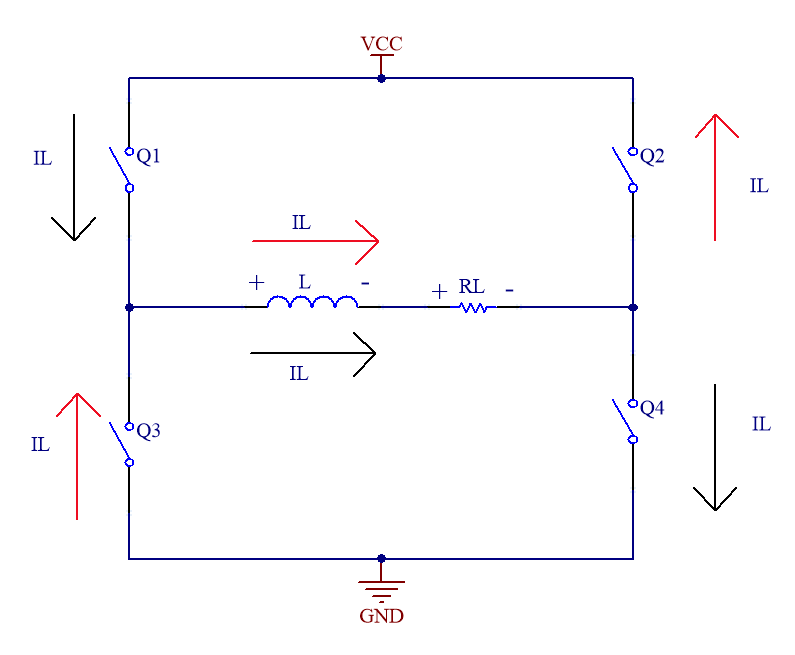
\includegraphics[scale=0.5]{puente_con_llaves.png}
	\caption{Topología simplificada de puente completo con cuatro llaves.}
	\label{fig:img_topologia_simplificada}
\end{figure} 


El electroimán se conecta entre los puntos medios de cada par de llaves. Cada una de ellas puede ser controlada de manera independiente mediante señales eléctricas. A través de una combinación correcta de las mismas se puede controlar la polaridad de la alimentación y el sentido de circulación de la corriente, según se desee. Para esta aplicación en particular, la fuerza magnética es siempre en el mismo sentido, independientemente del sentido en que circule la corriente. Por lo tanto, se adopta como sentido de circulación positivo de izquierda a derecha como lo indican las flechas en la figura \ref{fig:img_topologia_simplificada}. Por otro lado, es posible observar que la tensión con la que se alimenta al puente está representada por $V_{CC}$.

Para poder obtener una forma de onda de corriente como la que se muestra en la figura \ref{fig:img_corriente_exponencial}, comenzando desde corriente nula, se debe controlar el estado de las llaves de la siguiente manera:

\begin{itemize}
	\item En principio se cierran las llaves $Q_1$ y $Q_4$ a la vez, generando un circuito entre $V_{CC}$, el electroimán y GND como indican las flechas negras en la figura \ref{fig:img_topologia_simplificada}. De esta forma, la corriente comienza a crecer con forma de exponencial negativa. 
	\colorbox{red}{Habría que decir algo sobre ILmax? ej. corriente menor a la de reg. perm.?}
	\item Al llegar al límite superior de corriente ($I_{L_{MAX}}$), se debe conmutar el estado de las llaves, de manera que $Q_1$ y $Q_4$ dejen de conducir, y comiencen a hacerlo $Q_2$ y $Q_3$. De esta manera, la corriente seguirá circulando en el mismo sentido como indican las flechas rojas, pero ahora la diferencia de potencial en los bornes del electroimán se opone al paso de la corriente, por lo que su magnitud comienza a decrecer.
	\item Una vez alcanzado el límite inferior de corriente ($I_{L_{MIN}}$), se vuelve a conmutar el estado de las llaves para que la corriente vuelva a crecer.
	\item Este ciclo se repite en régimen permanente para que el valor medio de la corriente generada coincida con la deseada. 
\end{itemize}

%Si se elige un tiempo de conmutación pequeño comparado a la constante de tiempo de la planta, la fuerza magnética producida por esta corriente oscilante podrá ser filtrada, quedando únicamente su valor medio. Es decir, no habrá variaciones significativas en la fuerza ejercida.

Es importante tener en cuenta que sólo dos llaves pueden encenderse a la vez, y esto debe realizarse de manera diagonal. Es decir, en la figura \ref{fig:img_topologia_simplificada}, $Q_1$ y $Q_4$ pueden estar encendidos, mientras que $Q_3$ y $Q_2$ están apagados, y viceversa. Esto es debido a que se podría generar un cortocircuito entre la fuente de alimentación y GND, produciendo una circulación de corriente elevada que podría dañar el sistema y la fuente de alimentación. Se debe tener en cuenta esta restricción al momento de diseñar el circuito encargado de controlar estas llaves.

A diferencia del controlador mediante un transistor trabajando en modo lineal, en esta topología se logra una eficiencia extremadamente alta, ya que las llaves operan en corte y conducción, por lo que la disipación de potencia se produce solo en el electroimán y no en el circuito de control. Debido a este motivo, se decide implementar esta topología en el diseño de la fuente de alimentación.

\subsection{Diseño del lazo de control de corriente}

Como se mencionó previamente, para el diseño de la fuente de alimentación del electroimán se utilizará una topología de puente H trabajando en conmutación. Por lo tanto, para obtener el valor medio de corriente deseado es necesario controlar el tiempo que se le aplica cierta polaridad de tensión al electroimán. Para ello, se debe actuar sobre las llaves en función de si se desea que la corriente aumente o disminuya.

Una manera de implementar la lógica de control es mediante un controlador de lazo cerrado del tipo ON-OFF como se muestra en el diagrama en bloques de la figura \ref{fig:img_diag-en-bloques-comparador-sin-hist}. Este controlador realiza una resta entre la corriente de referencia y la corriente que está circulando por el electroimán, obteniendo una corriente de error ($I_e$). De esta forma, si la corriente medida es menor a la de referencia, la polaridad de la tensión aplicada en los bornes del electroimán será positiva para lograr que su corriente crezca e iguale a la de referencia. En cambio, si resulta mayor, la alimentación será negativa y la corriente disminuirá.

\begin{figure}[H]
	\centering
	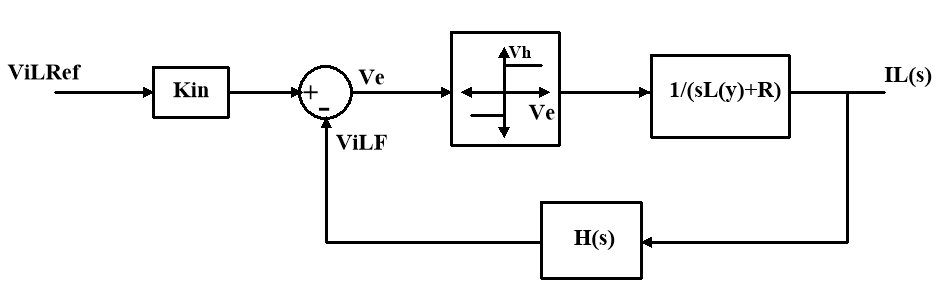
\includegraphics[width=\textwidth]{Diagrama-en-bloques-comparador-sin-hist.png}
	\caption{Diagrama en bloques simplificado del controlador de corriente.}
	\label{fig:img_diag-en-bloques-comparador-sin-hist}
\end{figure}



%Por otro lado, al considerar que el tiempo de conmutación es pequeño comparado a la constante de tiempo de la planta, la forma de onda de la corriente en régimen permanente será triangular puesto que no llegará a tomar forma exponencial. 

%Además, como la tensión aplicada a los bornes del electroimán en cada semiciclo de conmutación es igual en magnitud y el circuito de carga y descarga del electroimán es el mismo, la onda triangular tendrá pendientes simétricas. La forma de onda resultante se puede observar en rojo en la figura \ref{fig:img_corriente_triangular}.



Al analizar el diagrama en bloques planteado en la figura \ref{fig:img_diag-en-bloques-comparador-sin-hist} es posible notar que, una vez que la corriente del electroimán ($I_{L}(s)$) supere infinitesimalmente a la referencia, se producirá una conmutación en la polaridad de tensión aplicada al electroimán. Lo mismo sucede cuando es infinitesimalmente menor. El inconveniente que esto presenta es que se producirían conmutaciones extremadamente rápidas en torno al valor medio, por lo que sería necesario tener alta velocidad en conmutación. Por lo tanto, para reducir la frecuencia de esas oscilaciones, resulta conveniente agregar histéresis al controlador como se muestra en la figura \ref{fig:img_diag-en-bloques}.

\begin{figure}[H]
	\centering
	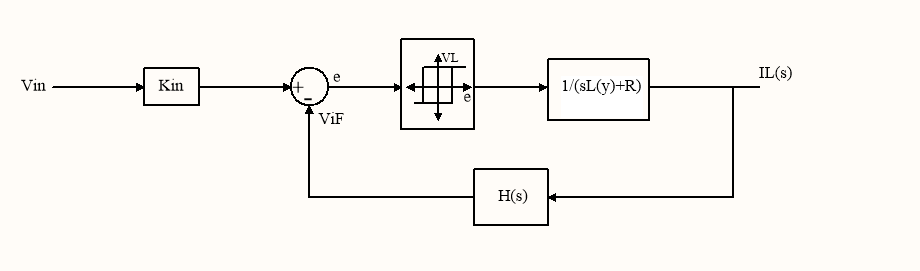
\includegraphics[width=\textwidth]{Diagrama-en-bloques.png}
	\caption{Diagrama en bloques del controlador de corriente con histéresis.}
	\label{fig:img_diag-en-bloques}
\end{figure}

\colorbox{red}{ver si conviene agregar deltaI en el diagrama}
\colorbox{red}{Esta bien que sea Vh la salida? Habría que unificar despues..}

La histéresis permite definir un margen de corriente $\Delta I_L$ de forma tal que, si la corriente que circula por el electroimán supera a la de referencia, no se producirá un cambio de polaridad en la tensión aplicada hasta que la supere por $\frac{\Delta I_L}{2}$. Análogamente, cuando comienza a decrecer, seguirá haciéndolo hasta que sea menor a la corriente de referencia menos $\frac{\Delta I_L}{2}$. La forma de onda de corriente resultante se puede observar en la figura \ref{fig:img_corriente_exponencial-hist}.

\begin{figure}[H]
	\centering
	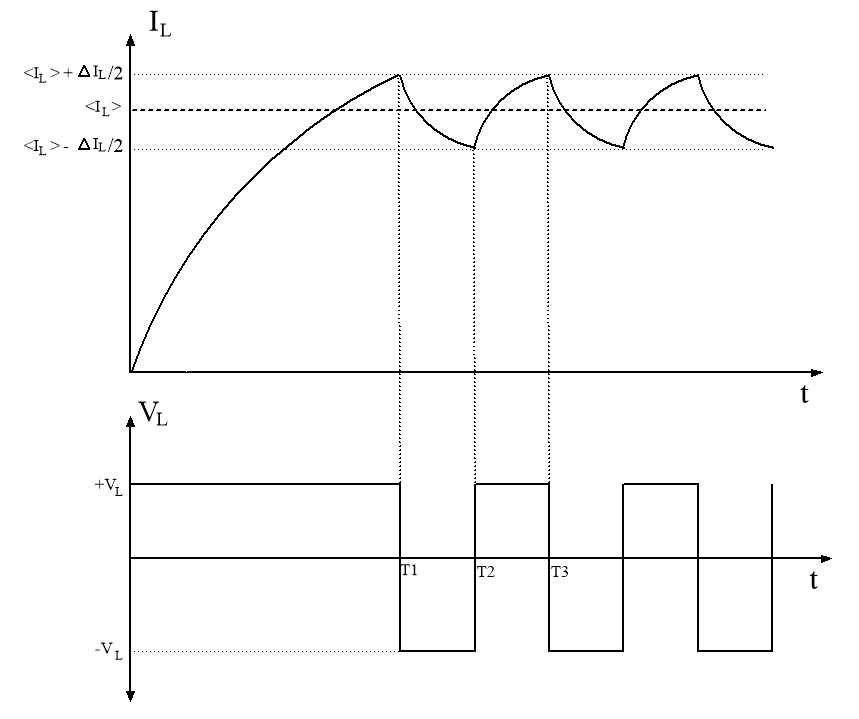
\includegraphics[scale=0.5]{Forma-de-onda-corriente-exponencial-hist.png}
	\caption{Forma de onda de corriente y tensión en el electroimán.}
	\label{fig:img_corriente_exponencial-hist}
\end{figure}



%\begin{figure}[H]
%	\centering
%	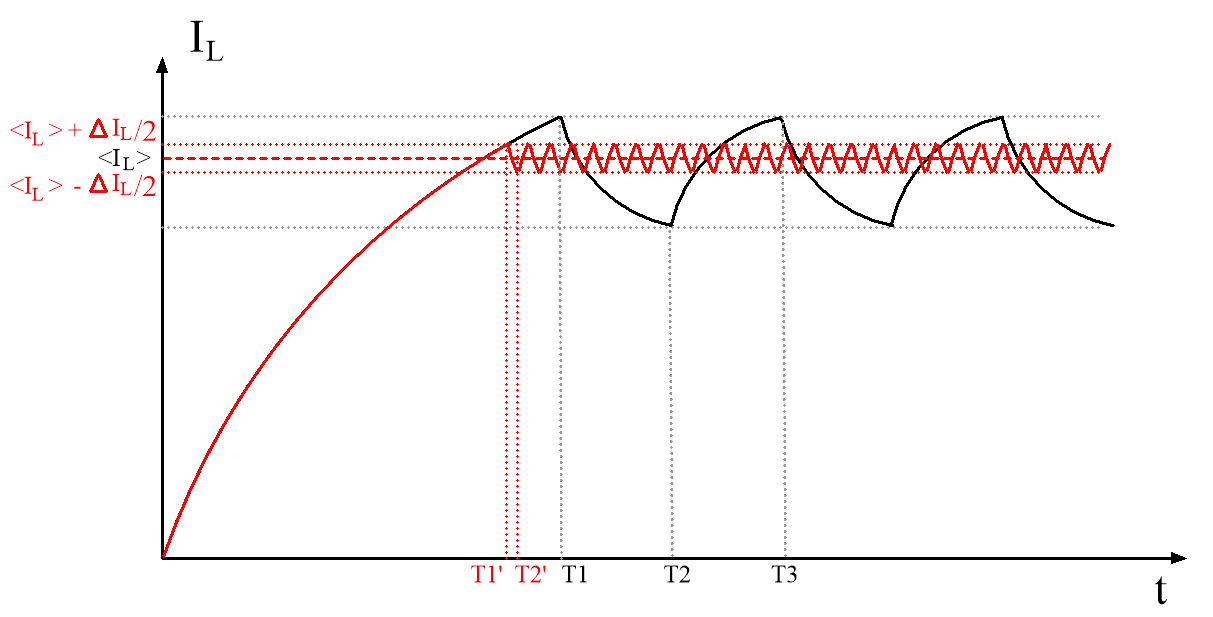
\includegraphics[scale=0.5]{Forma-de-onda-corriente-lineal.png}
%	\caption{Forma de onda de corriente triangular}
%	\label{fig:img_corriente_triangular}
%\end{figure} 

Debido a que lo único que cambia es la polaridad de la tensión con la que se excita al electroimán, la constante de tiempo del circuito no cambia. Esto da como resultado  que la corriente oscile sobre un valor medio con igual tiempo de crecimiento que de decrecimiento. Esta oscilación también es conocida como \textsl{ripple}. Su amplitud es fija y está determinada por el ancho de histéresis con el que se diseñe el controlador. 

\subsection{Medición de corriente}


Como se puede ver en el diagrama en bloques \ref{fig:img_diag-en-bloques}, para poder realizar el control es necesario medir la corriente que circula por el electroimán y actuar en consecuencia.


Para hacer esto se debe utilizar un sensor que permita una medición de corriente hasta, por lo menos, $30\:A$  y con un error máximo tolerable tal que permita actuar al comparador y no afecte al sistema. Además lo de la conmutación q dijo el gusti…

Los sensores de corriente trabajan en transresistencia, por lo tanto, se agrega el bloque H en el lazo de realimentación figura \ref{fig:img_diag-en-bloques-conH-y-Kin}. Ahora $V_{iL}=i_{L}*rm$. De esta forma ahora se está trabajando con tensiones por lo tanto la corriente de referencia se afecta por el bloque $K_{in}$ para obtener su equivalente en tensión. El bloque resultante es el siguiente:

\begin{figure}[H]
	\centering
	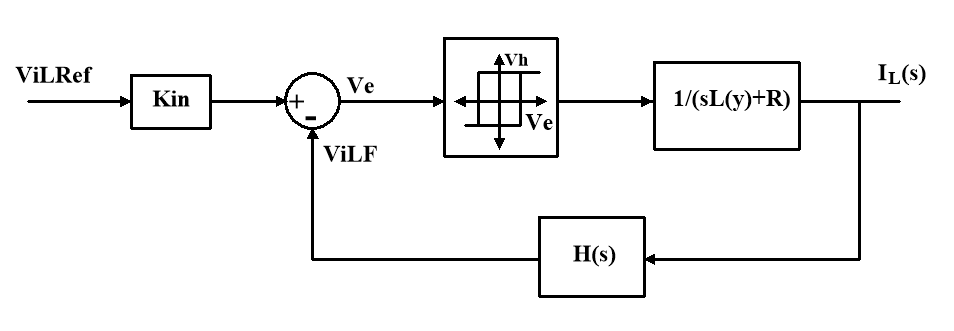
\includegraphics[width=\textwidth]{Diagrama-en-bloques-conH-y-Kin.png}
	\caption{Diagrama en bloques del controlador de corriente completo.}
	\label{fig:img_diag-en-bloques-conH-y-Kin}
\end{figure}

Se puede expresar al error que introduce el sensor de efecto hall como $V_{errSensor}$. Entonces la expresion de error $V_{e}$ resulta: 

\begin{equation}\label{eq_error_ve}
	V_{e}= K_{in}*I_{ref}-H*iL\pm V_{errSensor}=\triangle I \pm V_{errSensor}
\end{equation}


De esta forma, tomando el  caso extremo $K_{in}*I_{ref}=H*i_{L}$ el error obtenido $V_{e}=\pm V_{errSensor}$.
Es decir que el error es el propio error del sensor. Si se toma un ancho de histéresis mucho mayor al error máximo introducido por el sensor, este error no afectaría al sistema ya que seria despreciable a comparación del valor que deltaI debería alcanzar para que el comparador cambie de estado.

El error que introduce el sensor de efecto hall $V_{errSensor}$ debe ser mucho menor al ancho de histéresis del comparador.

-----------------SEPARADOR-------

\section{Cálculo de parámetros del controlador}
En esta sección se determinarán los parámertos críticos para el correcto funcionamiento del controlador de corriente.
\subsection{Cálculo de tensión de alimentación}

\subsection{Cálculo de sensor de sensor de corriente}
\subsection{Cálculo de ganancia de entrada}

Para comenzar el diseño circuital es importante determinar cómo será la alimentación del controlador de corriente. Para definirla se tendrá en cuenta la velocidad de respuesta de la planta que está determinada por su constante de tiempo ($\tau$). Es decir el sistema debe ser lo suficientemente rápido para modificar el valor medio de la corriente ante perturbaciones o cambios en el punto de operación. Un caso a analizar es cuando, en régimen permanente, se modifica bruscamente la carga que se esta levitando. En esta situación el sistema debe aumentar o disminuir la corriente de forma abrupta para evitar que el objeto se caiga. El caso de mayor exigencia se da cuando a una distancia máxima de referencia $Y_g=5\:mm$ se modifica de carga mínima ($1\:Kg$) a máxima ($30\:Kg$). Utilizando la ecuación XX se obtiene que la corriente para ambos casos es de:

\begin{equation}
	I_L(Y=5\:mm)[m=30\:Kg]=20.4\:A 
\end{equation}
\begin{equation}
	I_L(Y=5\:mm)[m=1\:Kg]=3.72\:A
\end{equation}

Como el polo dominante ya está definido por el circuito RL del electroimán, la velocidad con que el sistema pueda alcanzar un valor de corriente elevado está determinado por el valor de la fuente de alimentación. La expresión teórica de la corriente es: 

\begin{equation}
	I_L(t)=\frac{V}{R_L} + (I_o-\frac{V}{R_L})*e^{-\frac{t}{\tau}}
\end{equation}

Donde:
\begin{itemize}
	\item V es la tensión de alimentación, que puede tomar valores $+V_{cc}$ y $-V_{cc}$.
	\item $I_o$ es la corriente en el instante inicial.
	\item $\tau$ es la constante de tiempo del electroimán.
\end{itemize}

Para encontrar la expresion del tiempo que tarda la corriente en alcanzar el valor maximo de corriente imax se reemplaza I0=2,9 y se obtiene T1. Esto da:

\begin{equation}\label{eq_tiempo_de_subida}
	T1=-\tau*ln(\frac{V_{cc}-R*I_{max}}{V_{cc}-R*I_{0}})
\end{equation}

Cuando se modifique la carga del objeto ,es necesario que el tiempo de subida de corriente T1 sea mucho menor al tiempo en que la carga llegue a la distancia máxima que el sistema soporta $Y=5mm$ aprox (que corresponde a imax). Es decir que el objeto cae libremente un delta $\Delta Y= 1mm $. Utilizando la ecuación que calcula el tiempo (T) que tarda en desplazarse un objeto en caída libre una altura $\Delta Y$:

\begin{equation}
	T=\sqrt{\frac{2*\Delta Y}{g}}=rt{\frac{2*1mm}{9.81}}=14,27\:ms
\end{equation}

Finalmente reemplazando en \ref{eq_tiempo_de_subida} se obtiene: $Vcc>=21.6\:V$.

Se puede decir cuanto da T1 si tomamos 24V.

\subsection{Cálculo de ancho de histéresis}

Como se mencionó, se desea controlar la fuerza ejercida a partir del valor medio de la corriente. Por lo tanto, las variaciones en torno a dicho valor medio no deben generar variaciones significativas en la fuerza magnética. Por ello, se debe elegir un ancho de histéresis tal que la frecuencia de conmutación resultante sea filtrada por la dinámica de la planta. Un valor de al menos 100 veces mayor que la frecuencia del polo de la planta obtenida en \ref{eq_transferencia_planta_m} serìa suficiente. Este se ubica en $70\:r/s$, lo que resulta en que se debe conmutar a una frecuencia de $\omega_{sw}>=7000\:r/s$, y expresada en Hz resulta $F_{sw}>=1\:kHz$.


Por lo tanto, como la frecuencia mínima es $F_{sw}$, y considerando que el tiempo en que crece la corriente es igual al que decrece, se obtiene que el tiempo máximo que puede tener la sección creciente de la corriente es igual a $t_{max}=500\:us$. 

A partir de la expresión \ref{eq_corriente_temporal_cond_iniciales} se puede obtener el valor máximo de ripple cuando $t=t_{max}$, considerando que la corriente inicial es $I_{min}$ y que la corriente final es $I_{min}+\Delta I_L$

\begin{equation} \label{eq_delta_i}
	I_{min}+\Delta I_{L_{max}}=\frac{v_L}{R_L}+(I_{min}-\frac{v_L}{R_L})*e^{-\frac{t_{max}}{\tau}}
\end{equation}

De la ecuación \ref{eq_delta_i} se puede despejar el valor máximo que puede tener $\Delta I_L$. 

\begin{equation} \label{eq_delta_i_2}
	\Delta I_{L_{max}}=6.06*10^{-3}*(\frac{v_L}{R_L}-I_{min})
\end{equation}
\colorbox{red}{Cambiar VL por VCC, y ver imagen de altium}

Sabiendo que el controlador de corriente tendrá una corriente media variable entre 0 y 30 A, se debe satisfacer la expresión \ref{eq_delta_i_2} para cualquier $I_{min}$ dentro de ese rango. Por lo tanto se plantean dos casos: $I_{min}=0$ e $I_{min}=30$. Para el primer caso se llega a que $\Delta I_{L_{max}}=727\:mA$ y en el segundo $\Delta I_{L_{max}}=500\:mA$. Por lo tanto se elige un ancho de histéresis de $500\:mA$ ya que cumple las dos condiciones.


\section{Diseño del circuito}

Se realizará el diseño circuital de cada bloque planteado en la figura \ref{fig:img_diag-en-bloques-conH-y-Kin}.

\subsection{Diseño de puente H}

capaz acá entraría lo del calculo de la fuente de alimentación

Para el diseño del puente H se deben definir qué componente electrónico cumplirá la función de actuaar como llave, proporcionar su circuitería de control, hip, bootstrap, todo eso

Como se mencionó previamente, se utiliza una topología de puente completo con 4 llaves para alimentar el electroimán. Para realizar una implementación circuital de ella, es necesario elegir qué componente electrónico cumplirá el rol de llave. Además se debe diseñar la circuitería necesaria para el correcto funcionamiento de las llaves.

\subsubsection{Elección de llaves}

Entre los dispositivos semiconductores más utilizados para trabajar en conmutación se encuentran los transistores bipolares de juntura (BJT), transistores de efecto de campo metal-oxido semiconductor (MOSFET) y los transistores bipolares de compuerta aislada (IGBT). Cada uno de ellos posee características distintivas que lo hacen mas o menos apropiado para cada aplicación en particular.

Dados los requerimientos de corriente del dispositivo, la intención de reducir las pérdidas de potencia en las llaves y los requerimientos de velocidad de conmutación (\colorbox{red}{ESTO ES MEDIO CHAMULLO}), resulta apropiado elegir MOSFET para ser utilizados como llaves. 

Estos dispositivos funcionan generando una tensión en su gate que genera un canal de conducción de corriente entre su drain y source... Para utilizarlos se necesita implementar un driver apropiado.... Acá entra el HIP


\subsection{realimentacion}
capaz acá habría que poner lo del sensor de efecto hall?? y lo del operacional que hace la resta de vbias
asd


\subsection{etapa de entrada y restador}


Se plantea la etapa de entrada que consiste en la ganancia $K_{in}$ y el restador con la señal realimentada. Como se mencióno MAS ARRIBA, la etapa de entrada tiene una ganancia. Esta debe ser implementada con un circuito de operacionales.

La salida de esta etapa, al igual que la tensión de salida del sensor de efecto Hall, se polarizan en un punto de operación de $2.5\:V$ Para lograrlo se utiliza un circuito como el que se muestra en la figura \ref{fig:img_etapa-de-entrada}.


\begin{figure}[H]
	\centering
	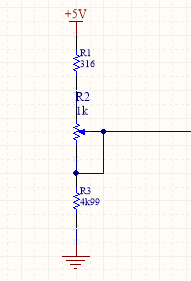
\includegraphics[scale=1]{Etapa-de-entrada.png}
	\caption{Etapa de entrada.}
	\label{fig:img_etapa-de-entrada}
\end{figure}
\colorbox{red}{Capaz sería mejor poner las imagenes directamente de Altium}

Las ecuaciones de diseño para este circuito son: ......


\subsection{comparador con histeresis}

Para la implementación del comparador con histéresis se utiliza un amplificador operacional realimentado positivamente. Se eligió que la corriente de salida del electroimán tenga un ripple de $500\:mA$. Por lo tanto, al afectar este valor por la transconductancia del sensor de efecto Hall, se obtiene un ancho de histéresis de $26.665\:mV$, alrededor de un punto de operación de $2.5\:V$. El circuito implementado se muestra en la figura \ref{fig:img_comp-con-hist}.

\begin{figure}[H]
	\centering
	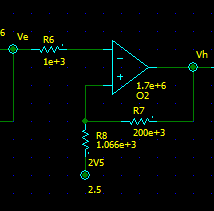
\includegraphics[scale=1]{Comparador-con-histeresis.png}
	\caption{Comparador con histéresis.}
	\label{fig:img_comp-con-hist}
\end{figure}

\subsection{conmutación auxiliar}
qqqwqw
\subsection{set-point de 2.6V}
 